% https://tex.stackexchange.com/questions/446948/how-to-place-a-parabola-distribution-on-top-of-a-node-in-tikz?rq=1
\documentclass[tikz,margin=2mm]{standalone}

\usepackage{tikz}

\tikzset{
    declare function={
        sig = 0.1;
        mu = 0;
        g(\x) = 1/(sig*sqrt(2*pi)) * exp(-1/2 * ((\x-mu)/sig)^2);
    }
}

\begin{document}

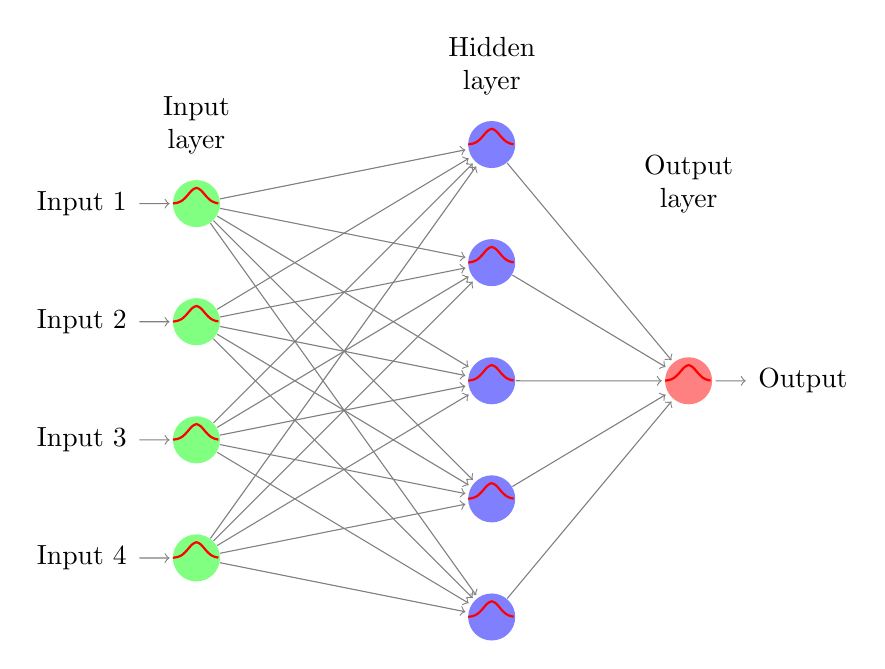
\begin{tikzpicture}[
    shorten >=1pt,
    ->,
    draw=black!50,
    node distance=2.5cm,
    scale=1.5,
    every pin edge/.style={<-,shorten <=1pt},
    neuron/.style={
        circle,fill=black!25,minimum size=17pt,inner sep=0pt,
        path picture={
            \draw[red,thick,-] plot[domain=-0.3:0.3,samples=11,smooth] ({\x},{0.05*g(\x)});
        },
    },
    input neuron/.style={neuron, fill=green!50},
    output neuron/.style={neuron, fill=red!50},
    hidden neuron/.style={neuron, fill=blue!50},
    annot/.style={text width=4em, text centered},
]

	% Draw the input layer nodes
	\foreach \name / \y in {1,...,4}
	% This is the same as writing \foreach \name / \y in {1/1,2/2,3/3,4/4}
	    \node[input neuron, pin=left:Input \y] (I-\name) at (0,-\y) {};
	
	% Draw the hidden layer nodes
	\foreach \name / \y in {1,...,5}
	    \path[yshift=0.5cm]
	        node[hidden neuron] (H-\name) at (2.5cm,-\y cm) {};
	
	% Draw the output layer node
	\node[output neuron,pin={[pin edge={->}]right:Output}, right of=H-3] (O) {};
	
	% Connect every node in the input layer with every node in the
	% hidden layer.
	\foreach \source in {1,...,4}
	    \foreach \dest in {1,...,5}
	        \path (I-\source) edge (H-\dest);
	
	% Connect every node in the hidden layer with the output layer
	\foreach \source in {1,...,5}
	    \path (H-\source) edge (O);
	
	% Annotate the layers
	\node[annot,above of=H-1, node distance=1cm] (hl) {Hidden layer};
	\node[annot,above of=I-1, node distance=1cm] {Input layer};
	\node[annot,above of=O] {Output layer};


\end{tikzpicture}

\end{document}